\subsection{Testing and Experimental Validation (Tomlin, Sastry, Lee, Karsai)}


The project team collaborated to create a Starmac simulation model, which was published on the web site. It was released as an example in the ESMoL tool distribution as well\cite{jp_esmol}.  Gabe Hoffman (Stanford) produced the original Starmac model in Simulink (Fig. \ref{fig:starmac_mdl}), which was later revised by Jim Kapinski (CMU) and then Nicholas Kottenstette (Vanderbilt).  The Vanderbilt team added passive controllers in the same architectural framework 
as the original Starmac controllers (Fig. \ref{fig:starmac_arch}).

\begin{figure}[thpb]
\centering
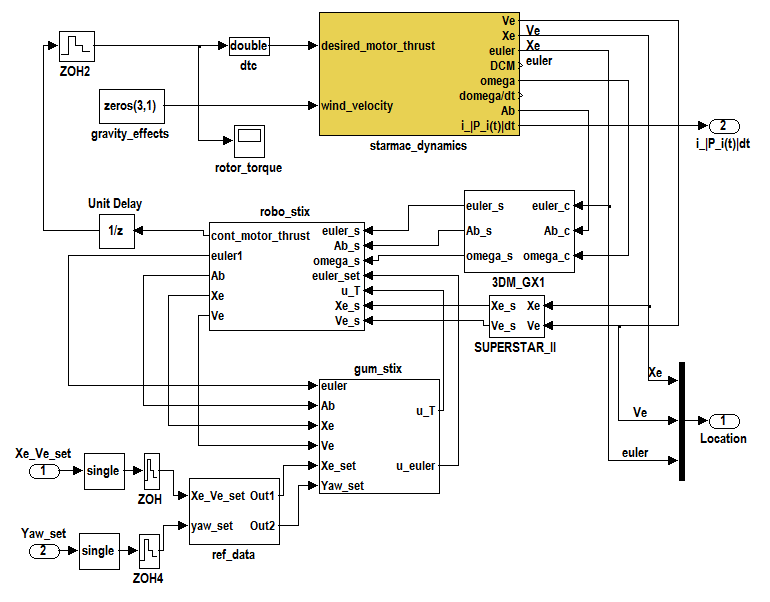
\includegraphics[width=0.9\textwidth]{img/real_quadrotor_mdl.png}
\caption{Simulink model of the Starmac quadrotor.}
\label{fig:starmac_mdl}
\end{figure}

\begin{figure}[thpb]
\centering
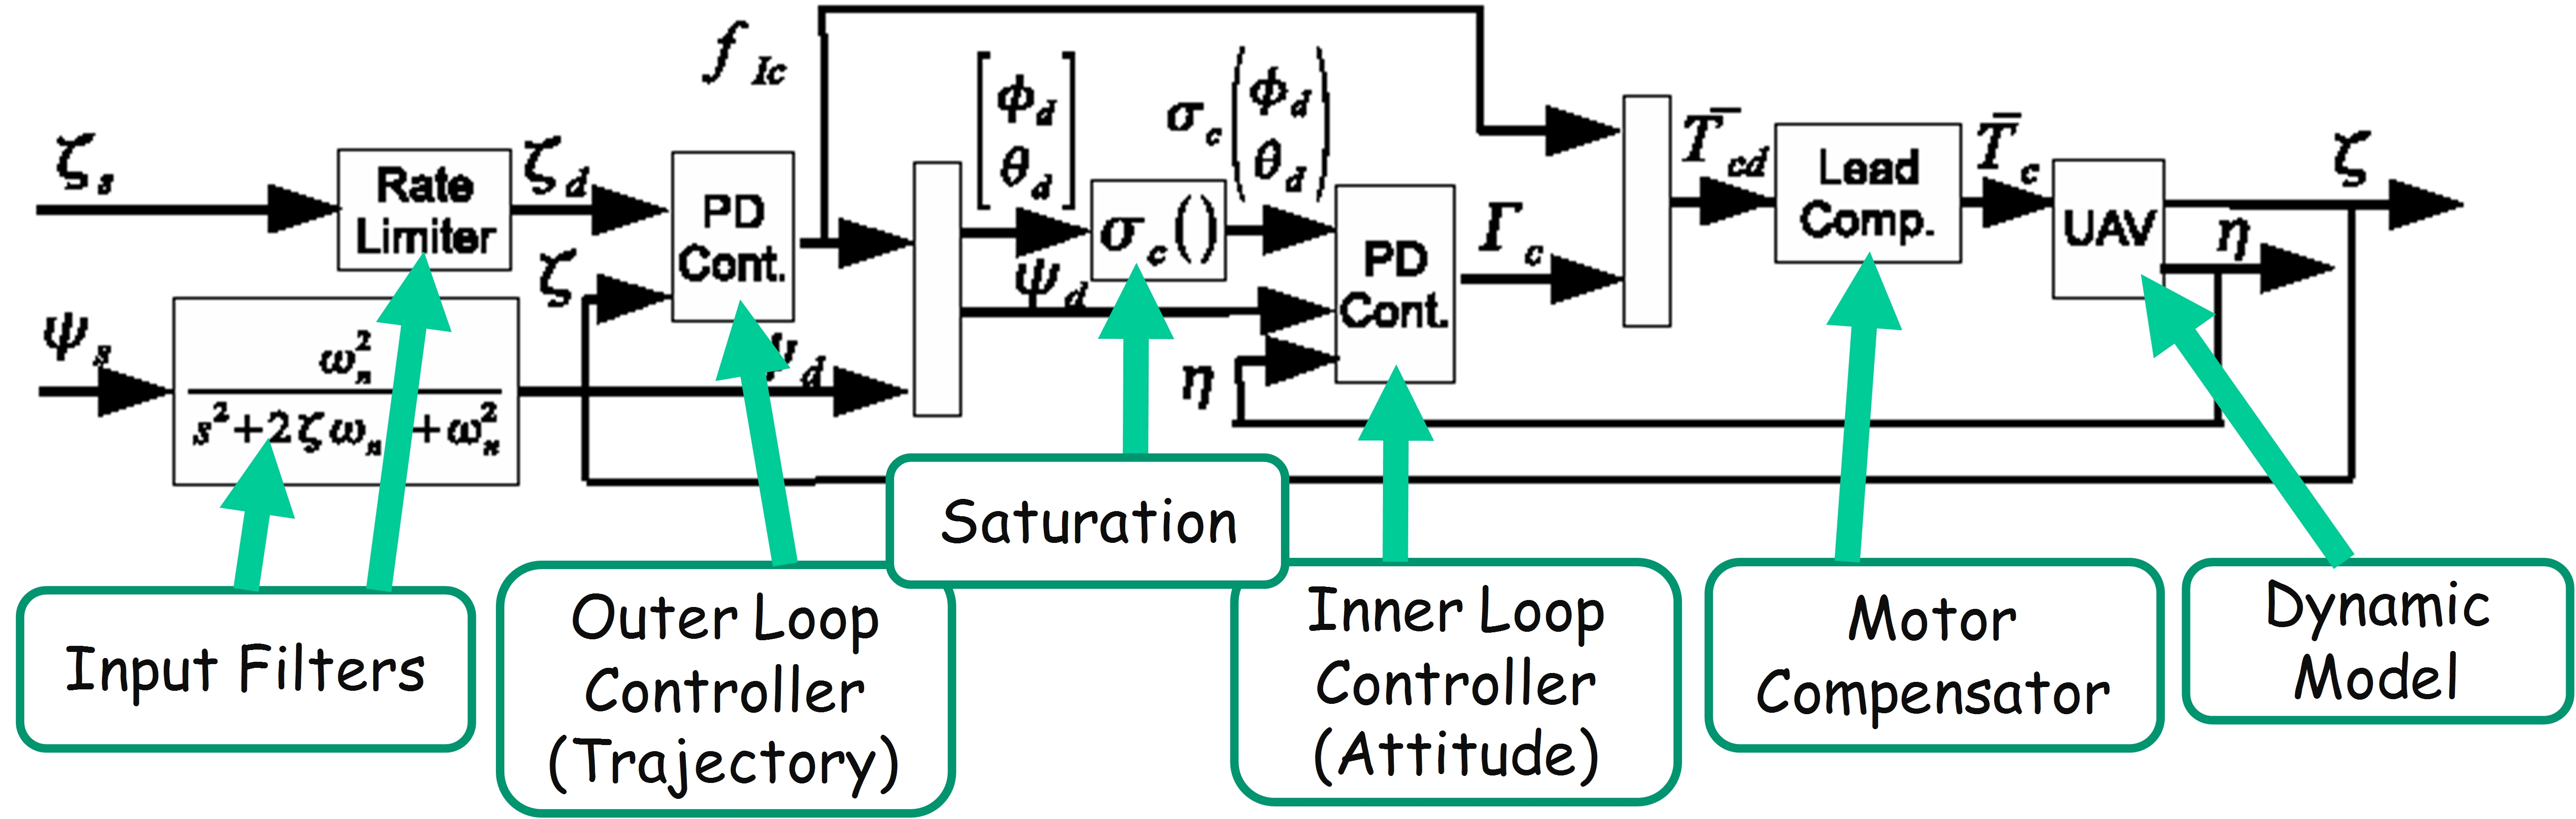
\includegraphics[width=0.9\textwidth]{img/quadrotor_arch.png}
\caption{Controller architecture for the quadrotor.}
\label{fig:starmac_arch}
\end{figure}

Beyond the evaluation in TrueTime described above, we also created a hardware-in-the-loop (HIL) experimental testbed to validate the controller code against the TrueTime models\cite{gh_truetime,nk_qr_tr,jp_dissertation}..
Fig. \ref{fig:hil_setup} contains the structure of the HIL experiment setup.  The xPC target software runs the quadrotor dynamics, and the actual Gumstix and Robostix processors run the passive controllers.  The interface between the plant simulator and the controller is ‘hard real-time’, and the xPC box simulates the real-time behavior of the plant with high-fidelity (e.g., inner loop control can be easily run at 100Hz).  The control software is generated and con-figured with the tool chain. Trajectories of the HIL-simulated controller appear in Fig. \ref{fig:starmac_hil}.

\begin{figure}[thpb]
\centering
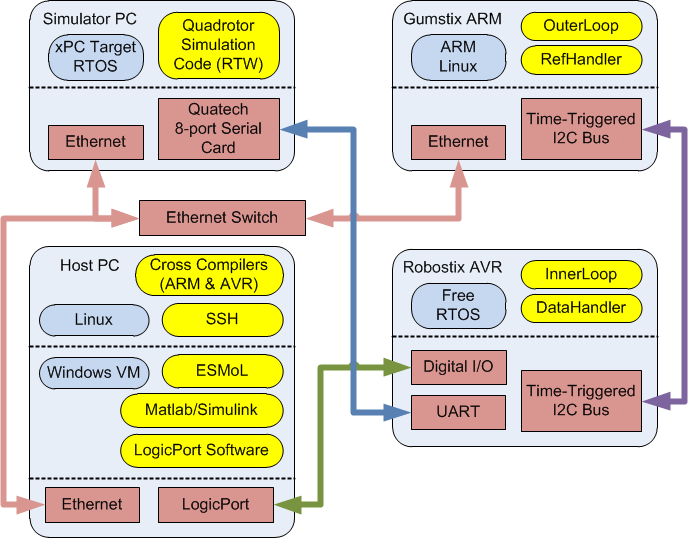
\includegraphics[width=0.9\textwidth]{img/hil_setup.png}
\caption{Overview of the hardware-in-the-loop simulation configuration.}
\label{fig:hil_setup}
\end{figure}


\begin{figure}[thpb]
\centering
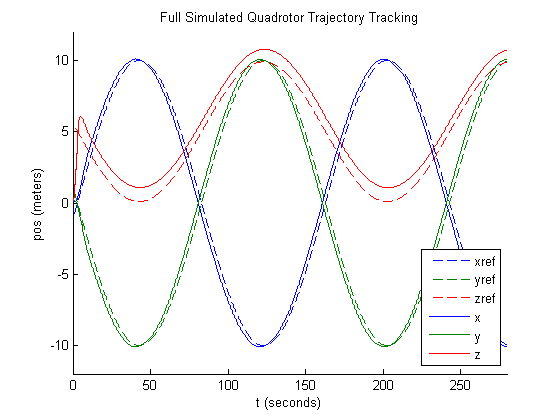
\includegraphics[width=0.9\textwidth]{img/qr_tracking.png}
\caption{Trajectory tracking for the passive controller code running in a hardware-in-the-loop simulation of the Starmac dynamics.}
\label{fig:starmac_hil}
\end{figure}


\emph{Online sector analysis}

We developed a moethod for comparing the stability criteria between the simulated quadrotor and its realization on the distributed network.
To illustrate the principle we used a continuous-time system whose model represents a simplified version of the quadrotor UAV.   This model still follows the  
basic component architecture for the control design (see Fig. \ref{fig:starmac_arch}), but excludes the nonlinear rotational 
dynamics of the full quadrotor while retaining
the difficult coupled stability characteristics.The 
example model controls a stack of four integrators (and motor lag) 
using two nested PD control loops.The two control loops (\emph{InnerLoop} and \emph{OuterLoop},
are deployed to the Robostix and Gumstix
processors, respectively, exactly as in the Starmac.  We refer to this example as the Quad Integrator model.  All of the controller components run at a frequency of 50Hz.  


Our controller evaluation method is based on sector theory, proposed originally by Zames to analyze nonlinear elements in a control design.  Sectors provide two real-valued parameters which represent bounds on the possible input/output behaviors of a control loop.  Kottenstette presented a sector analysis block for validating a control design in Simulink\cite{nk_qr_tr}.  We propose to use the same structure to verify the deployed quadrotor control software online.  This method is described more fully in Porter et al\cite{jp_online_stability}.  A few concepts make this approach appealing for our case:

\begin{enumerate}
 \item For a given component, the sector measures behavior simultaneously over multiple inputs and outputs, so only one sector analyzer is required per control loop.
 \item Our passive abstraction of the system design (described below) allowed us to use a sector analyzer for each control loop to quickly isolate problem components in the deployed design.
\end{enumerate}

Passive control requires that controllers use energy received from inputs or stored previously, introducing no new energy into the environment. If the plant dynamics were passive, we would have considerable freedom in setting gains and choosing control structures.  The zero-order hold outputs can introduce small amounts of new energy to the environment during rapid velocity changes, so each of the control loops must mitigate small amounts of ``active'' behavior.  The sector bound $a$ quantifies the energy-generating behavior of each control loop. In our quadrotor system, we expect the bound $a$ to be small and negative and choose the gains appropriately.  The result from Kottenstette indicates that the condition $k < -1/a$ is sufficient to ensure stability in these situations (where $k$ is the configured gain of the control loop)\cite{nk_qr_tr}.

\begin{figure*}[thpb]
\centering
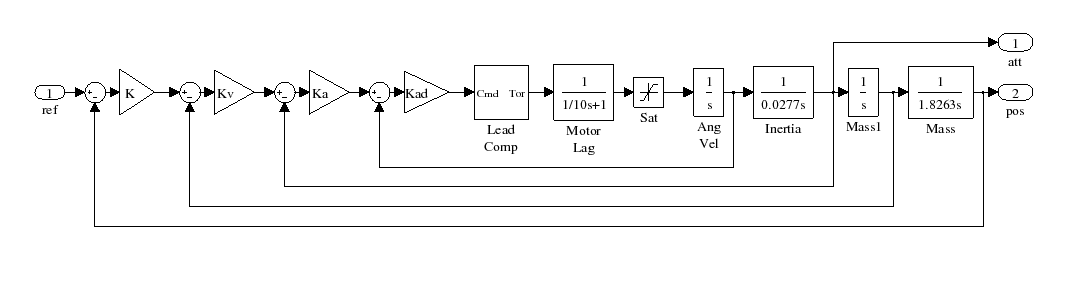
\includegraphics[width=\columnwidth]{img/quadrotor_loops}
    \caption{Conceptual nested loop structure of the controller.}
    \label{fig:quadrotor_loops}
\end{figure*}

This particular design must be evaluated from the innermost loop to the outermost loop in order to make sense of the gain constraints. Fig. \ref{fig:quadrotor_loops} shows the nested loop structure of the design.  The actual design and implementation are complicated by the physical architecture of the digital realization: 

\begin{enumerate}
 \item Sensors acquire digital attitude and position information only, so velocities must be estimated.
 \item The controller components are deployed to different processors in the digital implementation, as described previously. Components on the two processors exchange data messages using a time-triggered protocol.
 \item Motor thrust commands are issued periodically using a zero-order hold.  As discussed previously the hold introduces additional energy back into the environment, violating the passivity condition.
\end{enumerate}

The sector blocks are attached around each controller, so input and output ports are oriented from the point of view of the control element.  The output of the controller (input to the rest of the system) is connected to the sector analyzer input port.  The signal controlled by the controller (before the error term is formed) is part of the input to the controller, but from our point of view it is the output of the system, so it connects to the sector
analyzer output port.  Fig. \ref{fig:sectorconn} displays the connection of the sector search block around the position control gain for our example. $K_x$ is the proportional gain for the outer loop PD controller, and $K_v$ is the derivative gain.  

\begin{figure}[thpb]
\centering
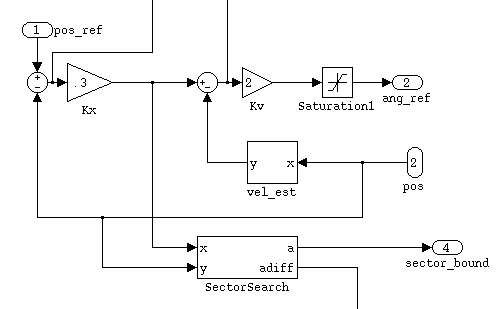
\includegraphics[width=0.75\columnwidth]{img/sectorconn}
    \caption{Sector analysis block (\emph{SectorSearch}) connection around the position controller.}
    \label{fig:sectorconn}
\end{figure}



\begin{figure}[thpb]
\centering
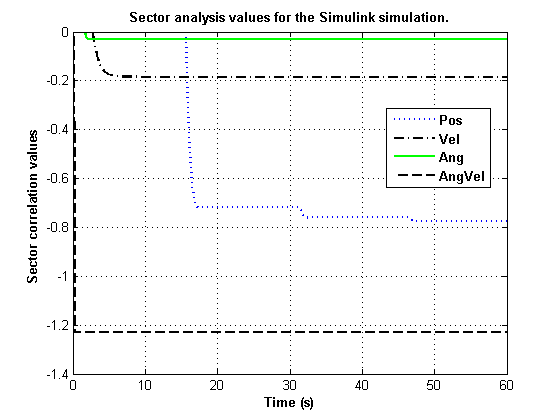
\includegraphics[width=0.75\columnwidth]{img/simsectors}
\caption{Sector value evolution over time for the quad integrator (Simulink only).}
\label{fig:sectors1} 
\end{figure}

\begin{figure}[thpb]
\centering
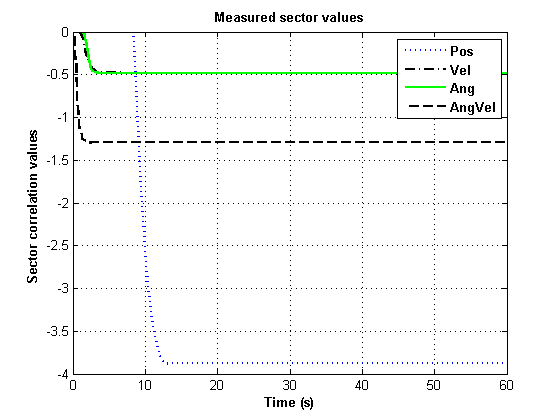
\includegraphics[width=0.75\columnwidth]{img/meassectors}
\caption{Sector value evolution over time for the quad integrator (Hardware-in-the-loop).}
\label{fig:sectors2} 
\end{figure}



\begin{table*}[thpb]
\centering

\begin{tabular}[width=0.95\columnwidth]{ | l | l | l | l | l | l | l | }

\hline
\textbf{Signal} & \textbf{Original} & \textbf{Simulated} & \textbf{Measured} & \textbf{Delta} & \textbf{New} & \textbf{New} \\
                & \textbf{Bound}    & \textbf{Sector}    & \textbf{Sector}  &                & \textbf{Bound} & \textbf{Sector} \\
\hline \hline
Angular  & -1.333 & -1.2292 & -1.2963 & -0.0671 & -2.667 & -1.4568 \\
Velocity & & & & & & \\
\hline
Angle & -0.5 & -0.0295 & -0.4831 & -0.4536 & -1.0 & -0.0068 \\
\hline
Velocity & -0.5 & -0.1856 & -0.4830 & -0.2974 & -1.0 &  -0.9324 \\
\hline
Position & -3.333 & -.7757 & -3.8811 & -3.1054 & -6.667 & -1.6081 \\
\hline
\end{tabular}
\caption{Sector value comparisons for simulation and execution on the actual platform.}
\label{tab:sectors}
\end{table*}




